\PassOptionsToPackage{unicode=true}{hyperref} % options for packages loaded elsewhere
\PassOptionsToPackage{hyphens}{url}
%
\documentclass[12pt,]{article}
\usepackage{lmodern}
\usepackage{amssymb,amsmath}
\usepackage{ifxetex,ifluatex}
\usepackage{fixltx2e} % provides \textsubscript
\ifnum 0\ifxetex 1\fi\ifluatex 1\fi=0 % if pdftex
  \usepackage[T1]{fontenc}
  \usepackage[utf8]{inputenc}
  \usepackage{textcomp} % provides euro and other symbols
\else % if luatex or xelatex
  \usepackage{unicode-math}
  \defaultfontfeatures{Ligatures=TeX,Scale=MatchLowercase}
    \setmainfont[]{Times New Roman}
\fi
% use upquote if available, for straight quotes in verbatim environments
\IfFileExists{upquote.sty}{\usepackage{upquote}}{}
% use microtype if available
\IfFileExists{microtype.sty}{%
\usepackage[]{microtype}
\UseMicrotypeSet[protrusion]{basicmath} % disable protrusion for tt fonts
}{}
\IfFileExists{parskip.sty}{%
\usepackage{parskip}
}{% else
\setlength{\parindent}{0pt}
\setlength{\parskip}{6pt plus 2pt minus 1pt}
}
\usepackage{hyperref}
\hypersetup{
            pdftitle={Analysis of arsenic and PFAS occurrence in community water systems in the United States},
            pdfauthor={Rachel Gonsenhauser},
            pdfborder={0 0 0},
            breaklinks=true}
\urlstyle{same}  % don't use monospace font for urls
\usepackage[margin=2.54cm]{geometry}
\usepackage{longtable,booktabs}
% Fix footnotes in tables (requires footnote package)
\IfFileExists{footnote.sty}{\usepackage{footnote}\makesavenoteenv{longtable}}{}
\usepackage{graphicx,grffile}
\makeatletter
\def\maxwidth{\ifdim\Gin@nat@width>\linewidth\linewidth\else\Gin@nat@width\fi}
\def\maxheight{\ifdim\Gin@nat@height>\textheight\textheight\else\Gin@nat@height\fi}
\makeatother
% Scale images if necessary, so that they will not overflow the page
% margins by default, and it is still possible to overwrite the defaults
% using explicit options in \includegraphics[width, height, ...]{}
\setkeys{Gin}{width=\maxwidth,height=\maxheight,keepaspectratio}
\setlength{\emergencystretch}{3em}  % prevent overfull lines
\providecommand{\tightlist}{%
  \setlength{\itemsep}{0pt}\setlength{\parskip}{0pt}}
\setcounter{secnumdepth}{5}
% Redefines (sub)paragraphs to behave more like sections
\ifx\paragraph\undefined\else
\let\oldparagraph\paragraph
\renewcommand{\paragraph}[1]{\oldparagraph{#1}\mbox{}}
\fi
\ifx\subparagraph\undefined\else
\let\oldsubparagraph\subparagraph
\renewcommand{\subparagraph}[1]{\oldsubparagraph{#1}\mbox{}}
\fi

% set default figure placement to htbp
\makeatletter
\def\fps@figure{htbp}
\makeatother

\usepackage{etoolbox}
\makeatletter
\providecommand{\subtitle}[1]{% add subtitle to \maketitle
  \apptocmd{\@title}{\par {\large #1 \par}}{}{}
}
\makeatother

\title{Analysis of arsenic and PFAS occurrence in community water systems in
the United States}
\providecommand{\subtitle}[1]{}
\subtitle{\url{https://github.com/rachel-gonsenhauser/Final_Project_Environmental_Data_Analytics}}
\author{Rachel Gonsenhauser}
\date{}

\begin{document}
\maketitle

\newpage
\tableofcontents 
\newpage
\listoftables
\newpage
\listoffigures 
\newpage

\hypertarget{rationale-and-research-questions}{%
\section{Rationale and Research
Questions}\label{rationale-and-research-questions}}

While the EPA establishes standards for 90 drinking water contaminants
by means of the federal Safe Drinking Water Act (SDWA) and its
regulations, public water systems still struggle to remain in compliance
with such policies (``Safe Drinking Water Act (SDWA)'', 2020). This
issue of compliance with the SDWA can stem from myriad causes, for
instance financial capacity of the water system. This is especially
concerning in areas where geologic conditions and/or anthropogenic
activities frequently introduce contaminants into drinking water
supplies. Additionally, many known contaminants still have yet to be
regulated by the EPA, such as poly- and perfluoroaklyl substances
(PFAS), which introduces even more complexity to the issue of water
quality monitoring of drinking water sources.\\
This analysis seeks to investigate the co-occurrence of water quality
indicators including arsenic, trihalomethane, uranium, and PFAS, which
originate from both geogenic and anthropogenic sources. Additionally,
given pervasive questions about how socioeconomic factors may be related
to water quality indicators, this analysis seeks to examine
relationships between drinking water contaminants and county-level
median household income (MHI) and size of the population served by a
given community water system (CWS). Additionally, questions regarding
how contaminant occurrences differ between states are explored.\\
To narrow the scope of this project, most analyses are targeted to
southeastern region states and northeastern region states. These regions
were chosen given their differences in climate, geology, and demographic
makeup. Additionally, individual case studies of Massachusetts and North
Carolina, selected following the data exploration phase, are explored in
further depth. As arsenic is present in much of the underlying geology
in many states in both regions, arsenic concentration data is the
predominant focus of analyses performed. Given that PFAS are emerging,
synthetic contaminants that have become the focus of many analyses in
the scientific community, PFAS data is also explored herein. Due to data
limitations, however, analyses using PFAS data are limited.

Specifically, the subsequent analyses explore the following questions:\\
\textbf{Question 1:} Do arsenic concentrations vary significantly from
state to state in southeastern and northeastern states?\\
\textbf{Question 2:} Do socioeconomic factors or the occurrence of other
contaminants predict arsenic concentrations in North Carolina and
Massachusetts?\\
\textbf{Question 3.} Are socioeconomic factors significant predictors of
PFAS concentrations?

\newpage

\hypertarget{dataset-information}{%
\section{Dataset Information}\label{dataset-information}}

Data used for this analysis were downloaded from the Centers for Disease
Control and Prevention (CDC)'s National Environmental Public Health
Tracking Network at \url{https://ephtracking.cdc.gov/DataExplorer/\#/}.
Output from this online tool containing geographic and CWS data
associated with individual variables was combined into the final
processed dataset used for this analysis.\\
The data wrangling process entailed taking individual datasets
containing data for arsenic, PFAS, uranium, trihalomethane, and MHI and
joining them into the final processed dataset. Each of these variables
had accompanying data inncluding the year, state, county, and CWS in
which the data was collected for each parameter. As unique county
Federal Information Processing Standards (FIPS) codes were standard
across all individual datasets, this variable was used to join datasets
into the final processed dataset. Following the generation of the
processed dataset, data were filtered to the appropriate level for each
analysis (e.g.~southeastern and northeastern region states).

\begin{quote}
\end{quote}

\begin{longtable}[]{@{}ll@{}}
\caption{Summary Information for Processed Dataset.}\tabularnewline
\toprule
Parameter & Summary\tabularnewline
\midrule
\endfirsthead
\toprule
Parameter & Summary\tabularnewline
\midrule
\endhead
Number of states & 28\tabularnewline
Number of CWSs & 25,583\tabularnewline
Water quality indicators & Arsenic, trihalomethane, uranium,
PFAS\tabularnewline
Socioeconomic variables & Population served by CWS, MHI\tabularnewline
Data collection time span & 1999-2018\tabularnewline
\bottomrule
\end{longtable}

\begin{longtable}[]{@{}lll@{}}
\caption{Description of Variables Used in Analyses.}\tabularnewline
\toprule
Variable & Description & Range\tabularnewline
\midrule
\endfirsthead
\toprule
Variable & Description & Range\tabularnewline
\midrule
\endhead
stateFIPS & Federal Information Processing Standard state code &
N/A\tabularnewline
State & state measurement was taken in & N/A\tabularnewline
countyFIPS & Federal Information Processing Standard county code &
N/A\tabularnewline
County & county measurement was taken in & N/A\tabularnewline
Year & year measurement was taken in & N/A\tabularnewline
Arsenic\_ugL & mean arsenic concentration (micrograms/liter) &
1-2,422\tabularnewline
PWS.ID & Public Water System Identification Number & N/A\tabularnewline
CWS.Name & Community Water System Name & N/A\tabularnewline
Population.Served & number of people served by CWS &
0-8,271,000\tabularnewline
MHI & median household income (\$) & \$16,435-\$113,336\tabularnewline
PFAS\_ppt & PFAS conncentration (parts per trillion) &
1-60\tabularnewline
TTHM\_ugL & mean trihalomethane concentration (micrograms/liter) &
0-219.20\tabularnewline
Uranium\_ugL & mean uranium concentration (micrograms/liter) &
0-379.10\tabularnewline
MCL\_TTHM & whether MCL for trihalomethanes is exceeded &
N/A\tabularnewline
MCL\_Uranium & whether MCL for uranium is exceeded & N/A\tabularnewline
MCL\_Arsenic & whether MCL for arsenic is exceeded & N/A\tabularnewline
\bottomrule
\end{longtable}

Table 1 provides a high level summary of the data provided in the
processed dataset. It should be noted that PFAS data was only available
for 2013-2015. For ease of analysis, this date range was changed to 2014
during the data wrangling process to create a common annual unit of
analysis for all variables. Table 2 provides descriptions of all
variables included in the processed dataset with data ranges provided
for continuous variables.

\newpage

\hypertarget{exploratory-analysis}{%
\section{Exploratory Analysis}\label{exploratory-analysis}}

While the distributions of all variables in the dataset were explored
during data wrangling and exploration, this section highlights key
results from the data exploration process. As research questions focus
on arsenic and PFAS concentrations, this exploratory analysis will
primarily explore data for these two variables.

\hypertarget{data-exploration-for-southeastern-states}{%
\subsection{Data Exploration for Southeastern
States}\label{data-exploration-for-southeastern-states}}

\begin{longtable}[]{@{}lll@{}}
\caption{Summary Statistics for Southeastern State
Variables.}\tabularnewline
\toprule
Parameter & Mean & Range\tabularnewline
\midrule
\endfirsthead
\toprule
Parameter & Mean & Range\tabularnewline
\midrule
\endhead
MHI & \$40,848 & \$16,435-\$92,097\tabularnewline
Population served by CWS & 14,893 people & 0-2,300,000
people\tabularnewline
Arsenic & 410.6 micrograms/liter & 1.0-2,395.0
micrograms/liter\tabularnewline
Uranium & 0.681 micrograms/liter & 0-23.84
micrograms/liter\tabularnewline
PFAS & 31.71 ppt & 7.0-59.00 ppt\tabularnewline
Trihalomethane & 17.47 micrograms/liter & 0-80.00
micrograms/liter\tabularnewline
\bottomrule
\end{longtable}

\begin{quote}
\end{quote}

Southeastern states examined experience a large range of income levels
and water system sizes; additionally, arsenic concentrations vary more
than any other contaminant examined (Table 3).

\begin{figure}
\centering
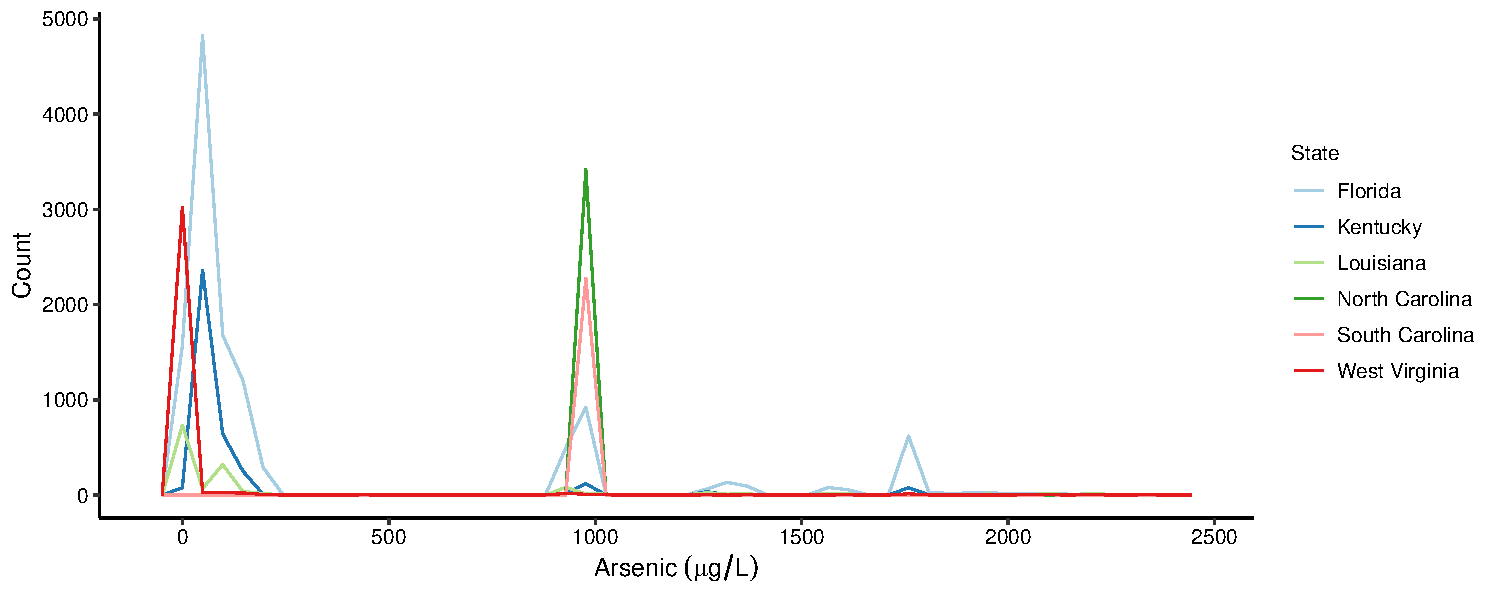
\includegraphics{Project_Template_files/figure-latex/figs-1.pdf}
\caption{Frequency of Arsenic Concentration Data in Southeastern
States.}
\end{figure}

West Virginia, Florida, Louisiana, and Kentucky all have relatively high
counts of arsenic observations at low concentration levels (Figure 1).
At the same time, North Carolina, South Carolina, and Florida have
relatively high counts of arsenic observations at higher concentrations
(around 1,000 micrograms/liter). This exploration of arsenic data in
southeastern states justifies an examination of how arsenic
concentrations vary among southeastern states and which explanatory
variables might predict arsenic concentrations.

\begin{figure}
\centering
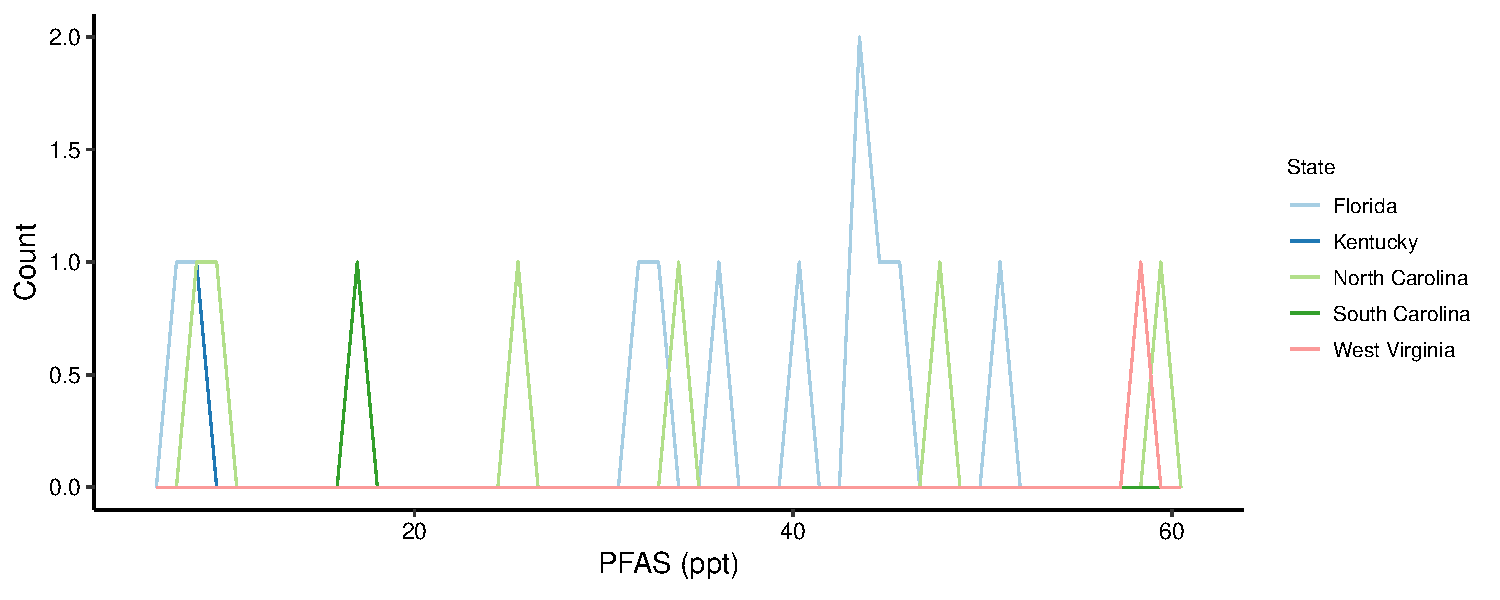
\includegraphics{Project_Template_files/figure-latex/figs2-1.pdf}
\caption{Frequency of PFAS Concentration Data in Southeastern States.}
\end{figure}

Compared to arsenic data, PFAS concentration data are far more limited
in southeastern states (Figure 2). The greatest frequency of counts
occurs in Florida at around 45 ppt with only two counts available. This
limitation of PFAS concentration data justifies a separate analysis of
PFAS data at a nationwide scale, as examining PFAS data regionally
severely limits the availability of data.

\newpage

\hypertarget{data-exploration-for-northeastern-states}{%
\subsection{Data Exploration for Northeastern
States}\label{data-exploration-for-northeastern-states}}

\begin{longtable}[]{@{}lll@{}}
\caption{Summary Statistics for Northeastern State
Variables.}\tabularnewline
\toprule
Parameter & Mean & Range\tabularnewline
\midrule
\endfirsthead
\toprule
Parameter & Mean & Range\tabularnewline
\midrule
\endhead
MHI & \$54,513 & \$26,323-\$113,336\tabularnewline
Population served by CWS & 13,791 people & 0-8,271,000
people\tabularnewline
Arsenic & 359.2 micrograms/liter & 1.0-2,2,422.0
micrograms/liter\tabularnewline
Uranium & 1.75 micrograms/liter & 0-43.00
micrograms/liter\tabularnewline
PFAS & 29.76 ppt & 3-60.00 ppt\tabularnewline
Trihalomethane & 10.37 micrograms/liter & 0-134.10
micrograms/liter\tabularnewline
\bottomrule
\end{longtable}

\begin{quote}
\end{quote}

Summary statistics for the northeastern United States indicate that the
mean MHI is higher than that in the southeast (Table 4). Additionally,
while the average water system size is similar across regions, the
northeast has systems that serve upwards of 8 million people, as
compared to a maximum size of 2 million people in the southeast (Tables
3 and 4). Ranges and average values for water quality indicators are
relatively similar in both regions (Tables 3 and 4).

\begin{figure}
\centering
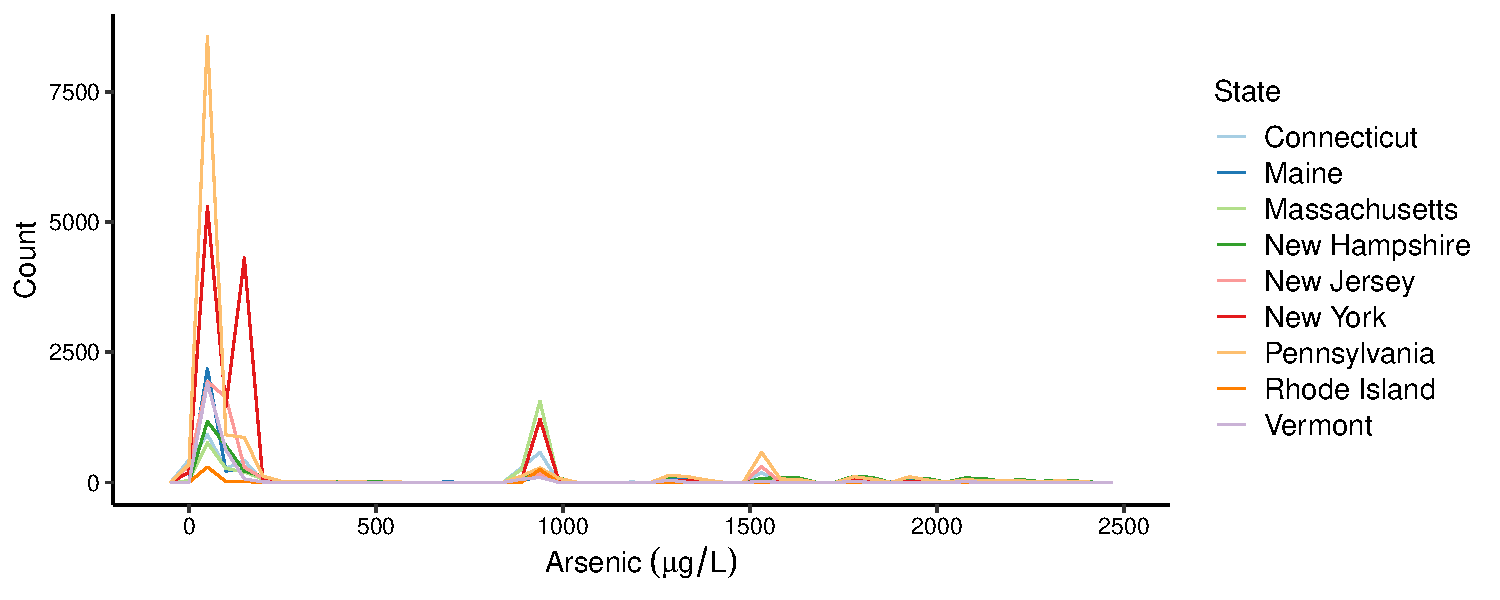
\includegraphics{Project_Template_files/figure-latex/figs3-1.pdf}
\caption{Frequency of Arsenic Concentration Data in Northeastern
States.}
\end{figure}

All northeastern states appear to have relatively high counts of arsenic
observations at low concentration levels, with New York and Pennsylvania
maintaining the greatest counts (Figure 3). Additionally, Massachusetts,
New York, and Connecticut, among other states also have many
observations at elevated arsenic concentrations (around 1,000
micrograms/liter). Similarly to southeastern states, this exploration of
arsenic data justifies a comparison of arsenic concentrations across
northeastern states. Additionally, understanding which explanatory
variables predict arsenic concentrations, particularly in states with
elevated levels, will be explored in the subsequent analysis performed.

\begin{figure}
\centering
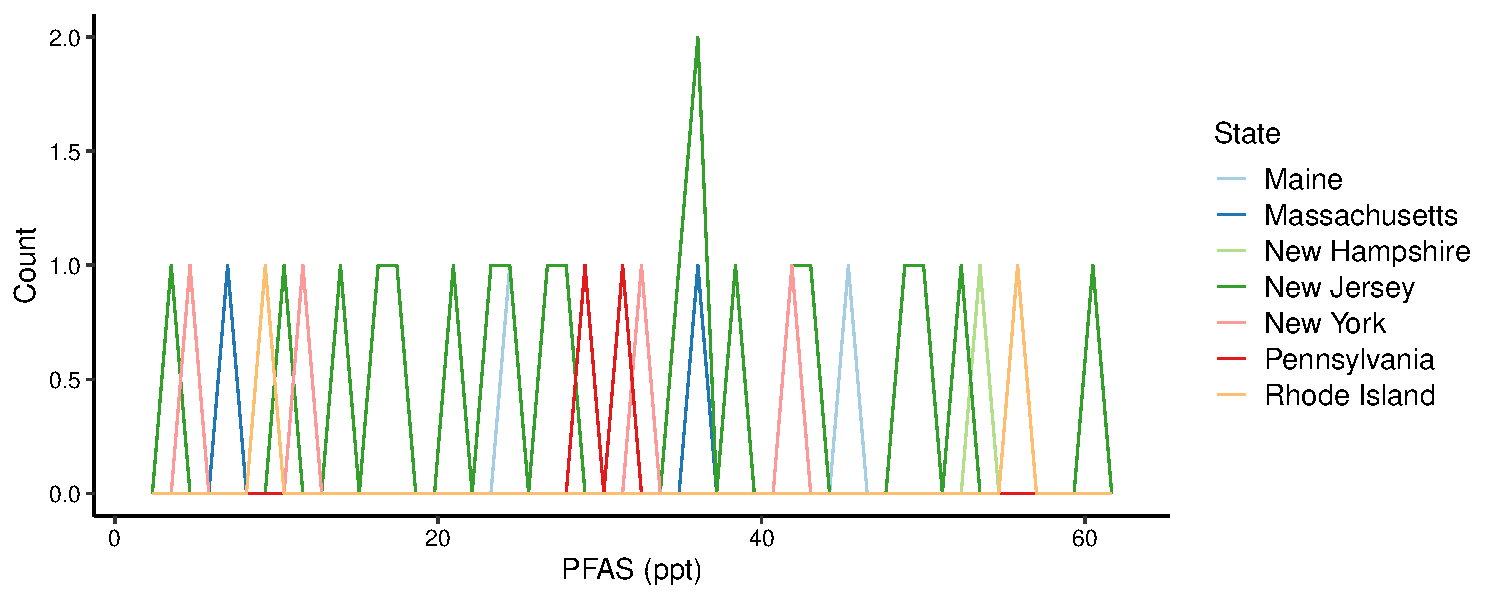
\includegraphics{Project_Template_files/figure-latex/figs4-1.pdf}
\caption{Frequency of PFAS Concentration Data in Northeastern States.}
\end{figure}

As in southeastern states, PFAS concentration data in northeastern
states are very limited (Figure 4). The largest frequency of counts
occurs in New Jersey at around 38 ppt with only two counts available.
Again, this data limitation provides rationale for examining PFAS data
on a nationwide scale, rather than regionally.

\newpage

\hypertarget{case-studies-data-exploration-for-north-carolina-and-massachusetts}{%
\subsection{Case Studies: Data Exploration for North Carolina and
Massachusetts}\label{case-studies-data-exploration-for-north-carolina-and-massachusetts}}

North Carolina and Massachusetts were selected as individual case
studies due to the prevalence of arsenic data at high concentrations
revealed earlier in the exploratory analysis. To gain insight into how
arsenic concentrations vary with respect to the variation of other
contaminants, arsenic, uranium, and trihalomethane data are provided for
both states across the data collection period (1999-2018).

\begin{figure}
\centering
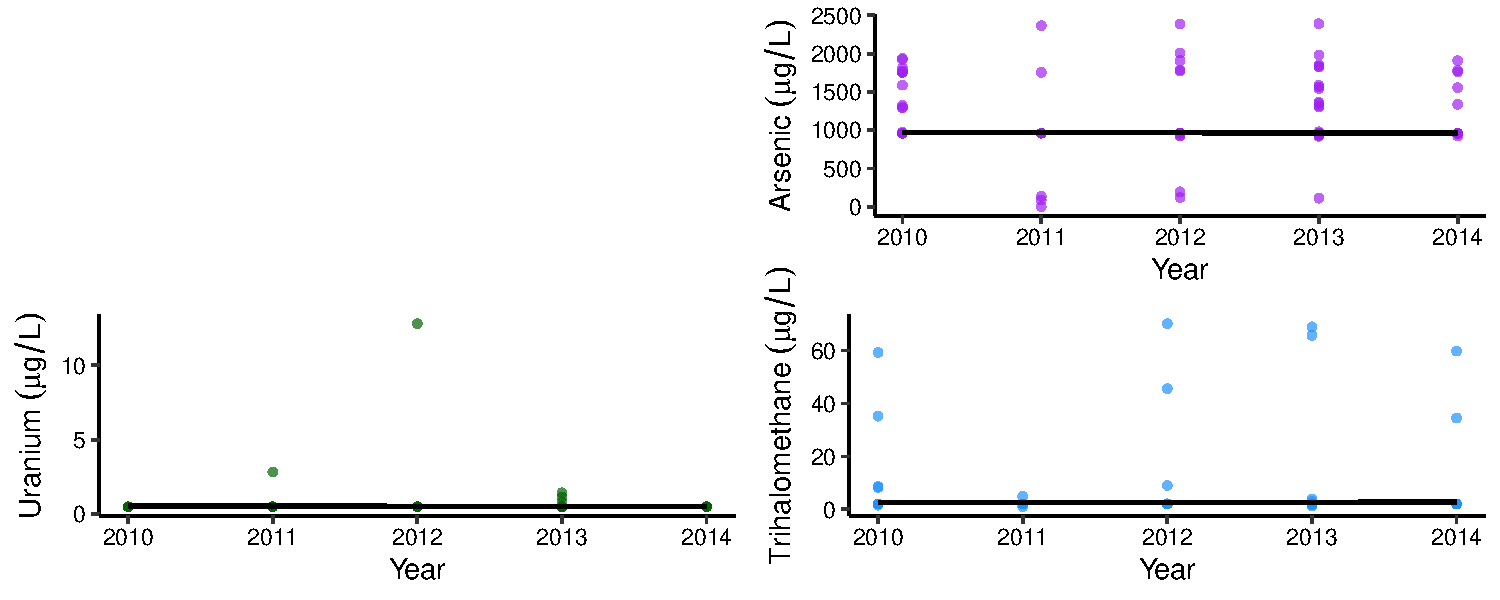
\includegraphics{Project_Template_files/figure-latex/figs5-1.pdf}
\caption{Water Contaminant Concentrations Over Time in North Carolina.}
\end{figure}

Over the period of 1999-2018 examined, North Carolina experiences
consistent levels of arsenic, uranium, and trihalomethane in CWSs
(Figure 5). The maximum cotaminant levels (MCL) for these three
contaminants, set by the US EPA, are 10 micrograms/liter, 30
micograms/liter, and 80 micrograms/liter respectively. As such, uranium
and trihalomethane concentrations in North Carolina over this period
remain safely below the MCL standard. Arsenic concentrations, however,
appear to occur well above the MCL for the entire period examined.

\newpage

\begin{figure}
\centering
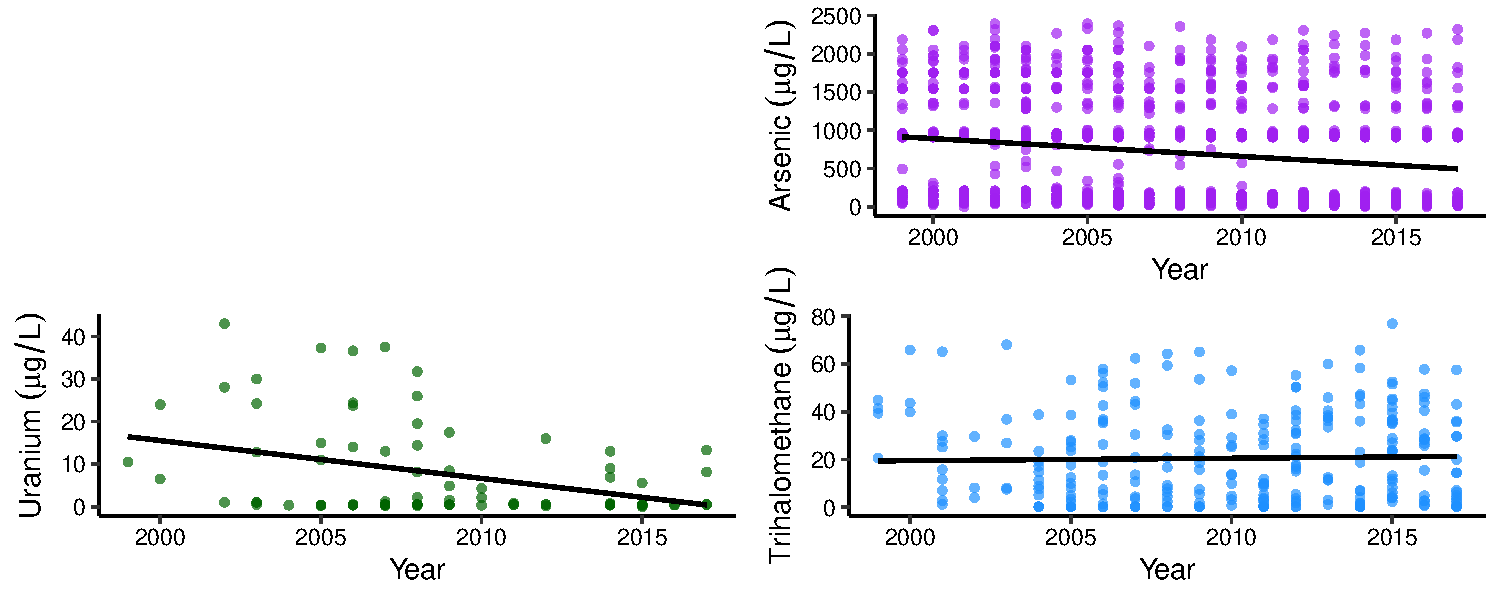
\includegraphics{Project_Template_files/figure-latex/figs6-1.pdf}
\caption{Water Contaminant Concentrations Over Time in Massachusetts.}
\end{figure}

Over the same period, Massachusetts experiences slightly declining
arsenic concentrations, substantially declining uranium concentrations,
and relatively constant trihalomethane concentrations (Figure 6).
Trihalomethane concentrations are safely below the MCL standard, as are
uranium concentrations from about 2010-2018. Conversely, arsenic
concentrations remain above the MCL for the entire 19-year period
examined.\\
This exploratory analysis has highlighted that arsenic concentrations
likely vary among states in the southeast and northeast and that
elevated arsenic levels occur in both North Carolina and Massachusetts.
As such, the subsequent analysis will focus primarily on examining
arsenic concentrations in these locations. Additionally, limited PFAS
data highlighted during this data exploration process motivates a
separate analysis of PFAS data in the subsequent section.

\newpage

\hypertarget{analysis}{%
\section{Analysis}\label{analysis}}

The following analysis seeks to answer the three questions stated at the
onset of this report. Key results of statistical analyses performed are
provided below.

\hypertarget{question-1-do-arsenic-concentrations-vary-significantly-from-state-to-state-in-southeastern-and-northeastern-states}{%
\subsection{Question 1: Do arsenic concentrations vary significantly
from state to state in southeastern and northeastern
states?}\label{question-1-do-arsenic-concentrations-vary-significantly-from-state-to-state-in-southeastern-and-northeastern-states}}

\begin{figure}
\centering
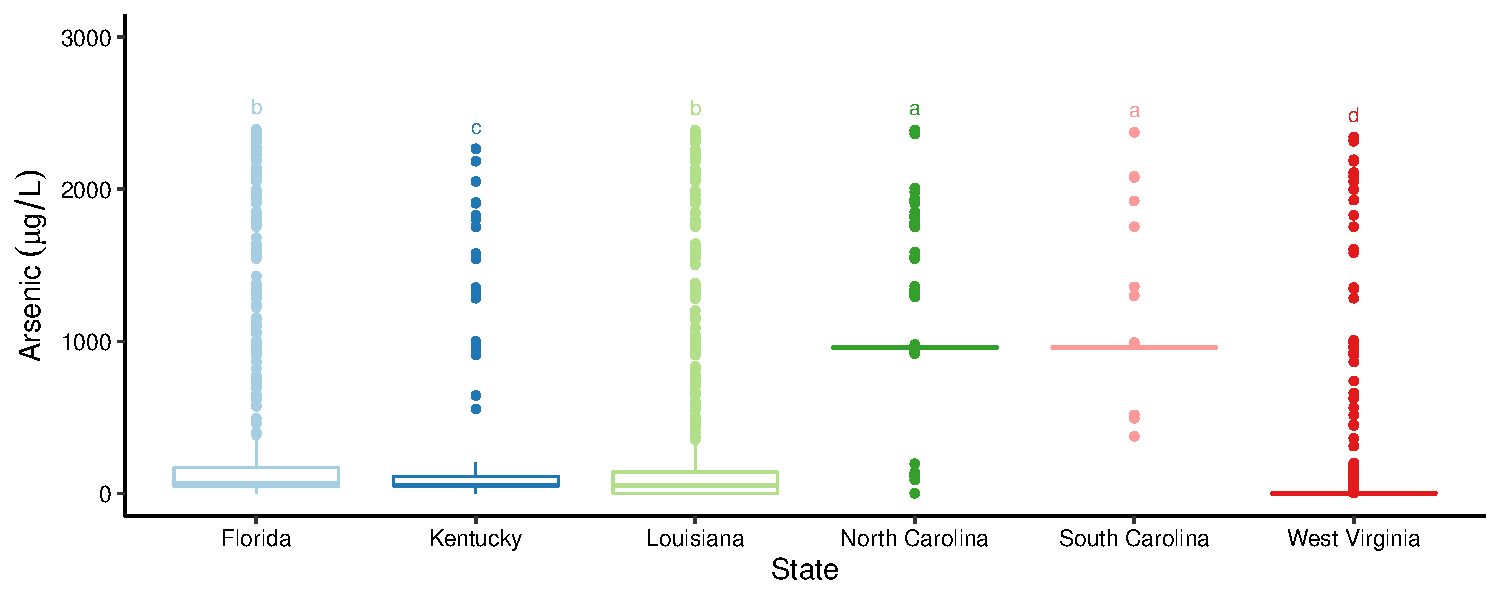
\includegraphics{Project_Template_files/figure-latex/figs7-1.pdf}
\caption{State by State Comparison of Arsenic Values for Southeastern
States.}
\end{figure}

Mean annual arsenic concentrations differ significantly between states
in the southeast (ANOVA; df=5, F=2872, p \textless{}0.0001). Arsenic
concentrations in West Virginia water systems were significantly lower
than those in other states and arsenic concentrations in North Carolina
and South Carolina were significantly higher than those in other states
(Post-hoc Tukey test; Figure 7).

\newpage

\begin{figure}
\centering
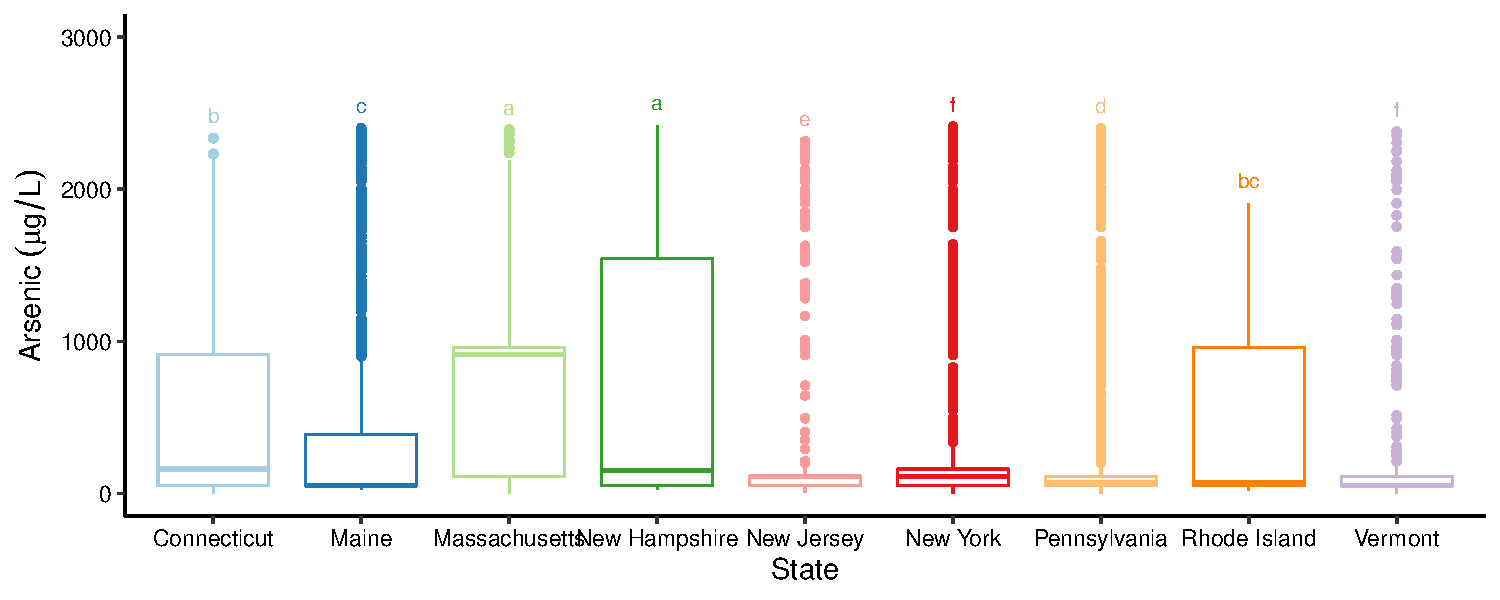
\includegraphics{Project_Template_files/figure-latex/figs8-1.pdf}
\caption{State by State Comparison of Arsenic Values for Northeastern
States.}
\end{figure}

Arsenic concentrations also differ significantly between states in the
northeast (ANOVA; df=8, F=630.9, p\textless{}0.0001). Arsenic
concentrations in New York and Vermont water systems were significantly
lower than those in other states while concentrations in New Hampshire
and Massachusetts were significantly higher than those in other states
(Post-hoc Tukey test; Figure 8).

\newpage

\hypertarget{question-2-do-socioeconomic-factors-or-the-occurrence-of-other-contaminants-predict-arsenic-concentrations-in-north-carolina-and-massachusetts}{%
\subsection{Question 2: Do socioeconomic factors or the occurrence of
other contaminants predict arsenic concentrations in North Carolina and
Massachusetts?}\label{question-2-do-socioeconomic-factors-or-the-occurrence-of-other-contaminants-predict-arsenic-concentrations-in-north-carolina-and-massachusetts}}

For both North Carolina and Massachusetts, uranium concentration was
explored as an explanatory variable but was ultimately removed from both
models for improved parsimony. For both states, final variables included
to explain variation in arsenic concentration are trihalomethane
concentration, MHI, and population served by the CWS.

\begin{figure}
\centering
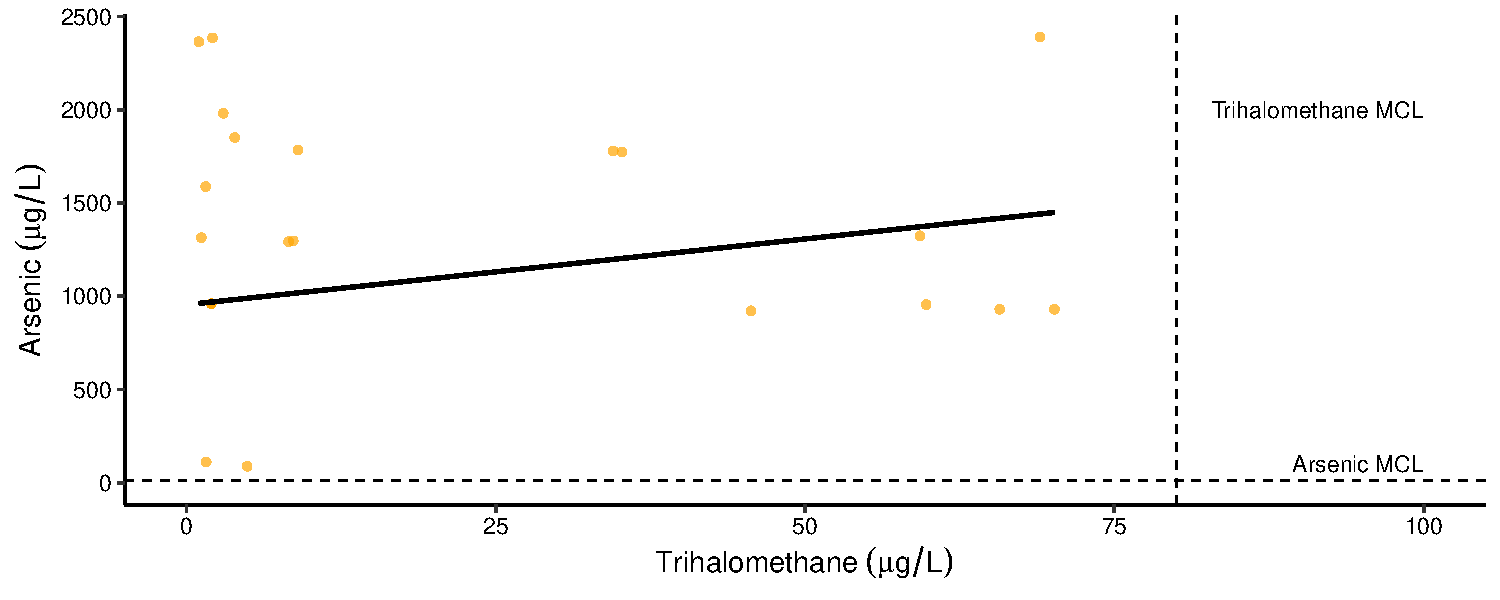
\includegraphics{Project_Template_files/figure-latex/figs9-1.pdf}
\caption{North Carolina Arsenic Concentrations by Trihalomethane
Concentration.}
\end{figure}

\begin{figure}
\centering
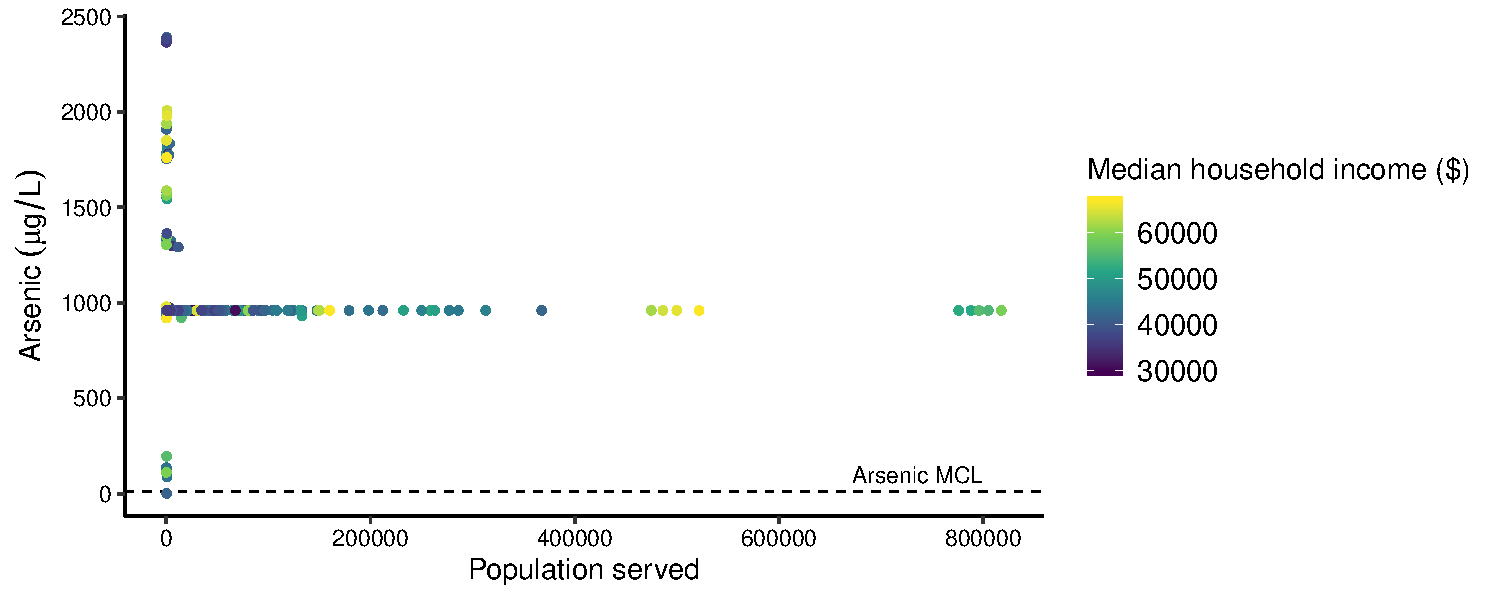
\includegraphics{Project_Template_files/figure-latex/figs10-1.pdf}
\caption{North Carolina Arsenic Concentrations by Population Served by
CWS Across Income Levels.}
\end{figure}

In North Carolina, population served by a CWS and trihalomethane
concentration significantly predict arsenic concentration, whereas MHI
is not a significant predictor of arsenic concentration (Multiple linear
regression; df=3 and 654, F=34.74, p\textless{}0.0001). Inreasing
arsenic concentration is associated with increasing trihalomethane
concentration (Figure 9) and with decreasing population size served by a
CWS (Figure 10). Additionally, there is no discernible relationship
between arsenic concentration and MHI (Figure 10). These results again
confirm that while trihalomethane concentrations remain below the EPA's
MCL threshold, arsenic levels are highly elevated in North Carolina
(Figures 9 and 10).

\begin{figure}
\centering
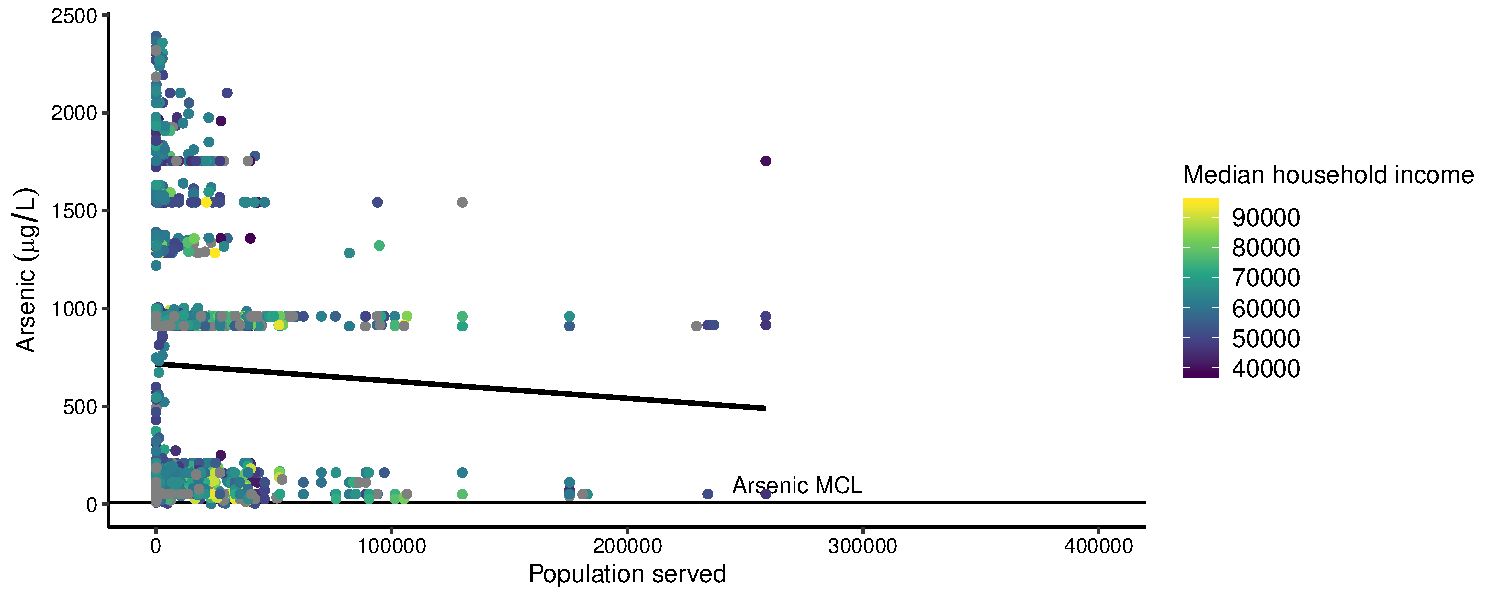
\includegraphics{Project_Template_files/figure-latex/figs11-1.pdf}
\caption{Massachusetts Arsenic Concentrations by Trihalomethane
Concentration.}
\end{figure}

\begin{figure}
\centering
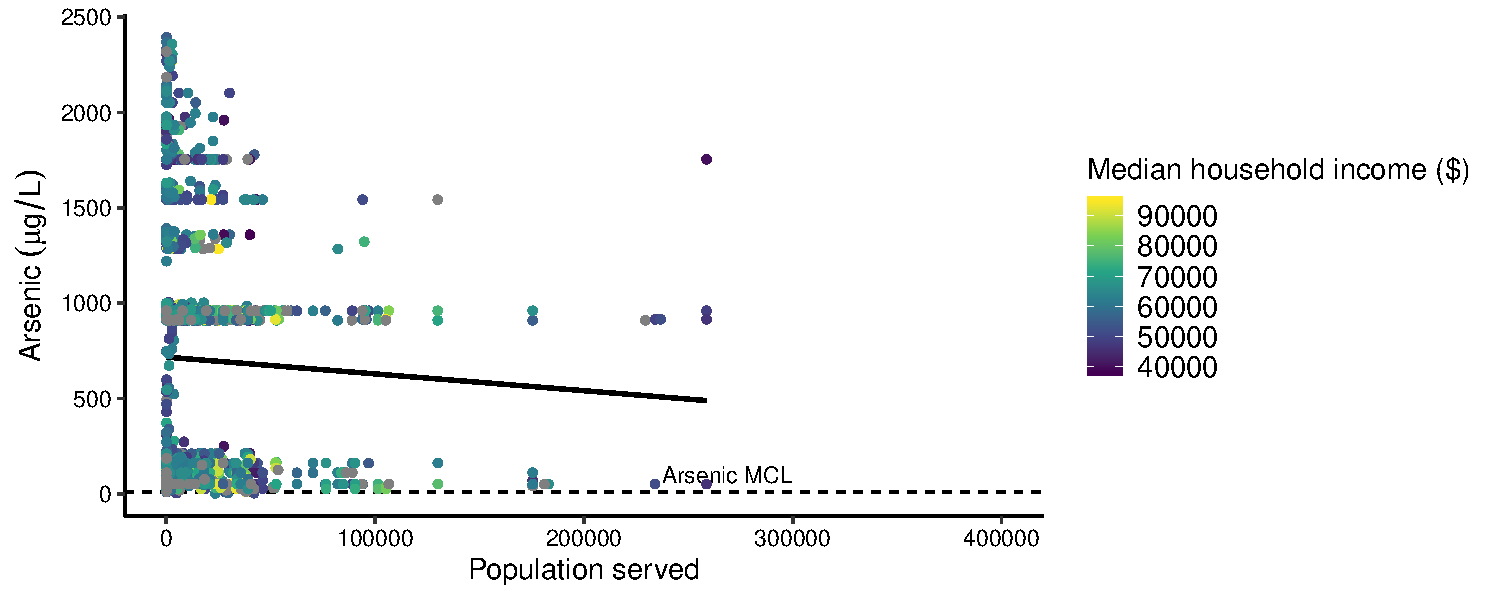
\includegraphics{Project_Template_files/figure-latex/figs12-1.pdf}
\caption{Massachusetts Arsenic Concentrations by Population Served by
CWS Across Income Levels.}
\end{figure}

In Massachusetts, neither population served by a CWS, trihalomethane
concentration, nor MHI significantly predict arsenic conncentration
(Multiple linear regression; df=3 annd 242, F=1.664, p=0.1753). While
there appears to be a slightly negative relationship between
trihalomethane and arsenic concentrations in Massachusetts, this
relationship is not significant (Figure 11). Additionally, a large range
of arsenic concentrations is experienced both across different
population sizes served by CWSs and across MHI levels (Figure 12). Like
in North Carolina, this analysis further confirms highly elevated
arsenic levels in Massachusetts, far above the EPA's MCL threshold of 10
micrograms/liter (Figures 11 and 12).

\begin{quote}
\end{quote}

\hypertarget{question-3.-are-socioeconomic-factors-significant-predictors-of-pfas-concentrations}{%
\subsection{Question 3. Are socioeconomic factors significant predictors
of PFAS
concentrations?}\label{question-3.-are-socioeconomic-factors-significant-predictors-of-pfas-concentrations}}

\begin{figure}
\centering
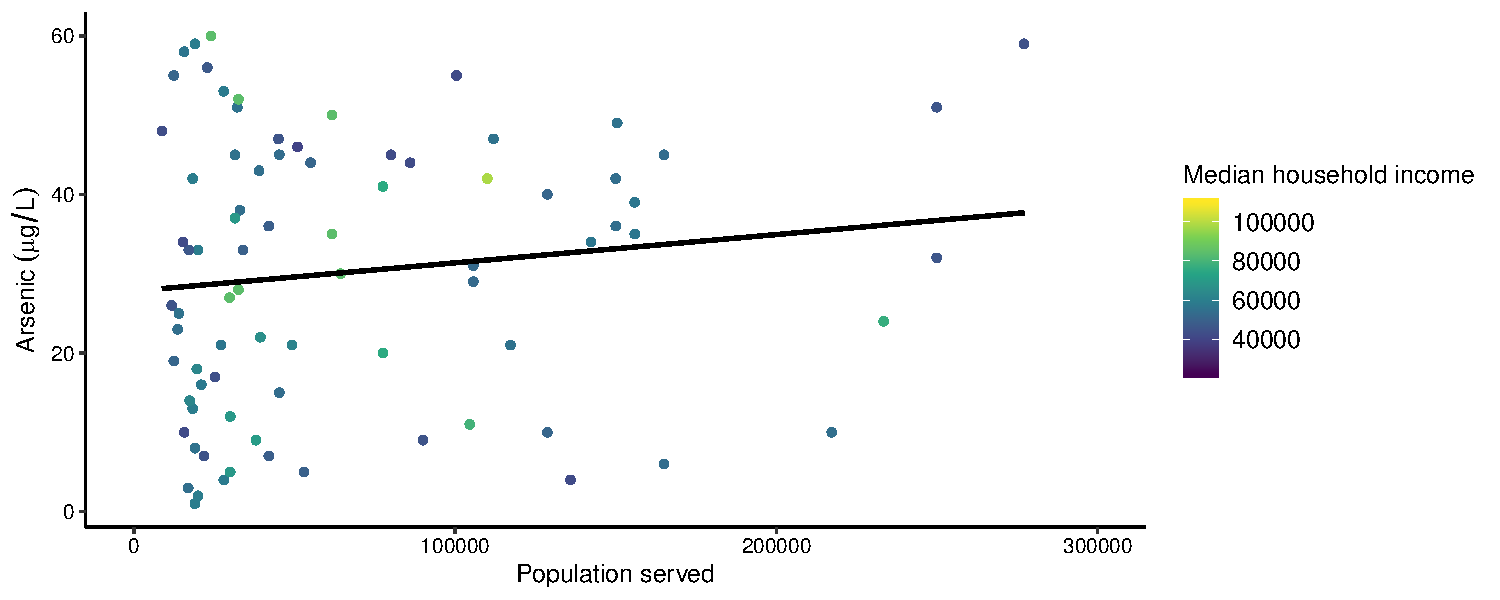
\includegraphics{Project_Template_files/figure-latex/figs13-1.pdf}
\caption{PFAS Concentration by Population Served by CWS Across Income
Levels.}
\end{figure}

Neither MHI nor population served by a CWS significantly predict PFAS
concentrations (Multiple linear regression; F=2 and 86, F=0.5912,
p=0.5559). PFAS concentrations vary widely across the size of the
population served by CWSs and across MHI levels (Figure 13). As the EPA
does not currently regulate PFAS, there is not an MCL guideline by which
to compare occurrence data.\\
An ANOVA was also run in preliminary analyses conducted for PFAS data,
but results are not included herein due to issues of missingness (25,938
observations were deleted upon running ANOVA).

\newpage

\hypertarget{summary-and-conclusions}{%
\section{Summary and Conclusions}\label{summary-and-conclusions}}

\hypertarget{arsenic-conclusions}{%
\subsection{Arsenic Conclusions}\label{arsenic-conclusions}}

This analysis reveals that among southeastern states, North Carolina and
South Carolina have significantly higher arsenic values than other
states in the region and that in the northeast, New Hampshire and
Massachusetts have significantly higher arsenic concentrations than
other states in the region. These findings are likely due to the
underlying geology in these states, as there are major arsenic hot spots
running through all four of these states (Figure 14).

\begin{figure}
\centering
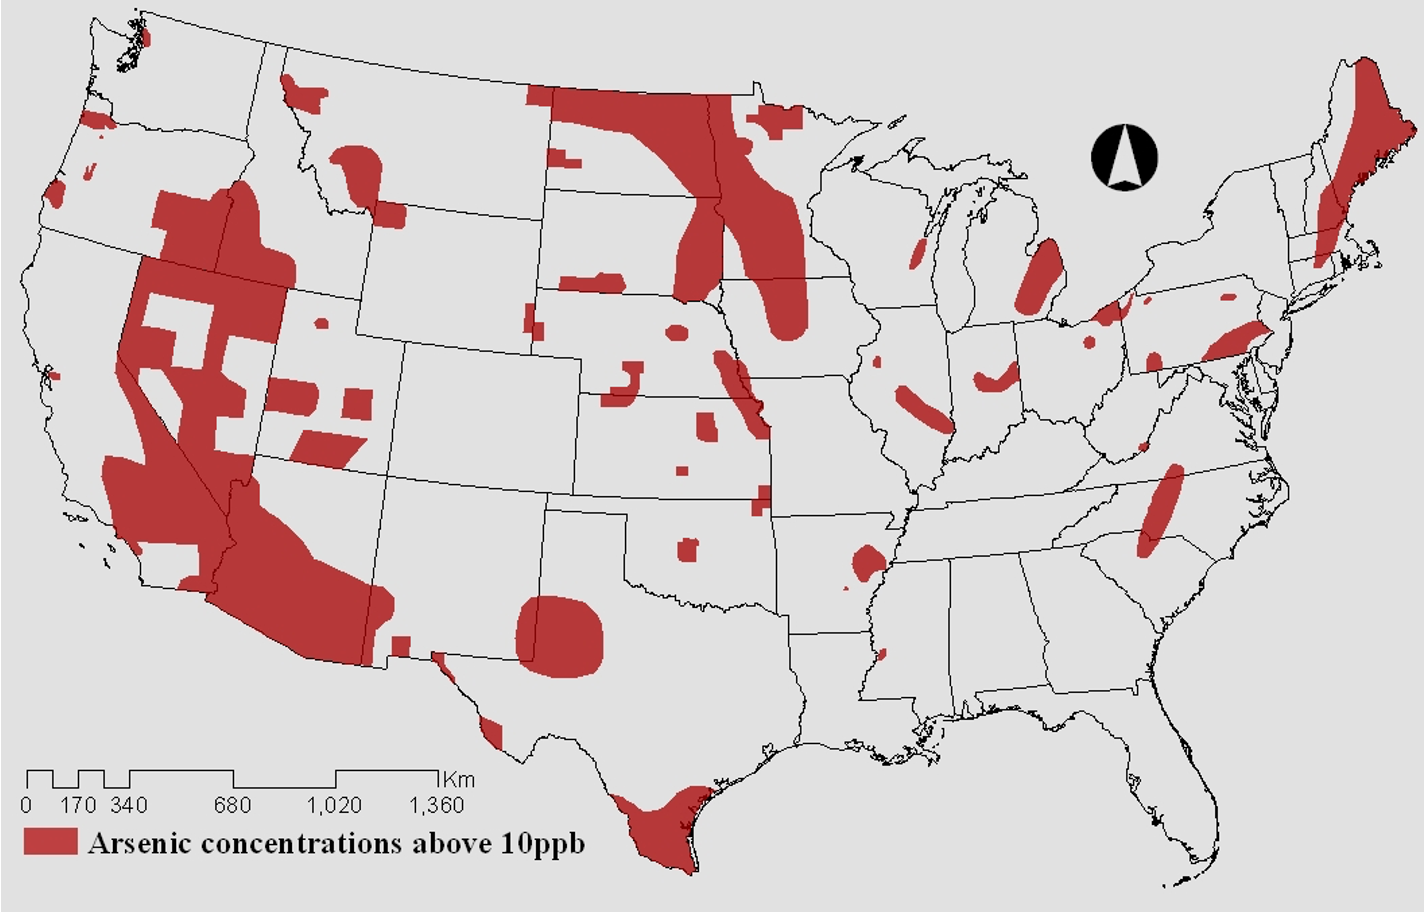
\includegraphics{../Data/Processed/ArsenicFigure.png}
\caption{Arsenic Occurrence in the United States, Source: Avner
Vengosh's lab, Duke University.}
\end{figure}

Whereas in Massachusetts no explanatory variables significantly
predicted arsenic concentrations, in North Carolina, trihalomethane
concentrations and the size of the population served by the CWS
significantly predicted arsenic concentrations. As trihalomethane is
often formed as a byproduct when treating water, it is logical that
arsenic and trihalomethane concentrations appear to co-occur in North
Carolina, as higher arsenic levels in drinking water likely trigger
higher rates of water treatment by water systems.\\
It is likely that arsenic concentrations increase with smaller
population size served by a CWS as smaller water systems are often
located in more rural areas and typically have less financial resources
at their disposal, often correspondinng with higher incidences of SDWA
violations. Additionally, it is possible that some of these smaller
water systems are not even regulated under the SDWA, as only public
water systems with 15 service connections or that serve 25 people per
day for 60 days of the year fall under SDWA jurisdiction and thus must
bring arsenic levels under the EPA'S MCL threshold (``Understanding the
Safe Drinking Water Act'', 2004).\\
While MHI was hypothesized to correlate with arsenic concentration, it
is possible that the lack of a significant relationship between these
variables is due to the pervasive occurrence of arsenic in the
underlying geology where high occurrences are noted. As such, arsenic
concentrations in drinking water would not necessarily be tied to a
county's MHI. In future analyses, the relationship between MHI and other
water contaminants that typically originate from anthropogenic sources,
rather than geogenic sources, should be explored.

\hypertarget{pfas-conclusions}{%
\subsection{PFAS Conclusions}\label{pfas-conclusions}}

Likely due to the limited data available, no explanatory variables
significantly predicted PFAS concentration. In February 2020, the EPA
issued a preliminary determination to regulate PFAS, particularly PFOA
and PFOS (``EPA Announced Proposed Decision to Regulate PFOA and PFOS in
Drinking Water'', 2020). The commencement of rulemaking efforts by the
EPA will likely increase the availability of PFAS data available as,
once a regulatory requirement is in place, data collection associated
with testing and mitigation will likely pick up. Once more data becomes
available, future analyses could focus on looking at similar
relationships explored here, or relationships between the occurrence of
PFAS and that of other contaminants.

\hypertarget{limitations-of-analysis}{%
\subsection{Limitations of Analysis}\label{limitations-of-analysis}}

Aside from the data limitation mentioned previously, another limitation
of this analysis stems from omitted variable bias, or the omission of
explanatory variables from models examined that may help to explain
variation in chosen response variables. Adjusted R-squared values for
all models geenrated were quite low (the highest of which was
approximately 0.13 for the model explaining arsenic concentrations in
North Carolina). This suggests that very little of the variation in
arsenic concentrations in drinking water is explained by the model. For
instance, a major omitted variable likely includes arsenic
concentrations in bedrock. Future analyses are necessary to further
understand which other variables may best explain this variation.

\newpage

\hypertarget{references}{%
\section{References}\label{references}}

\begin{enumerate}
\def\labelenumi{\arabic{enumi}.}
\tightlist
\item
  United States Environmental Protection Agency (USEPA). 2020. Safe
  Drinking Water Act (SDWA). Retrieved from:
  \url{https://www.epa.gov/sdwa}.
\item
  United States Environmental Protection Agency (USEPA). 2004.
  Understanding the Safe Drinking Water Act. Retrieved from:
  \url{https://www.epa.gov/sites/production/files/2015-04/documents/epa816f04030.pdf}.
\item
  United States Environmental Protection Agency (USEPA). 2020. EPA
  Announces Proposed Decision to Regulate PFOA and PFOS in Drinking
  Water. Retrieved from:
  \url{https://www.epa.gov/newsreleases/epa-announces-proposed-decision-regulate-pfoa-and-pfos-drinking-water}.
\end{enumerate}

\end{document}
